\newpage
\section{Status på Program} 
\label{sec:status_p_program}



Dette afsnit har til formål at konkludere på programmets status. Der blev skrevet et program fordelt på 52 C\# kodefiler og 13 designfiler. En liste over disse filer, kan findes i \cref{cha:filliste}. 

\begin{figure}
  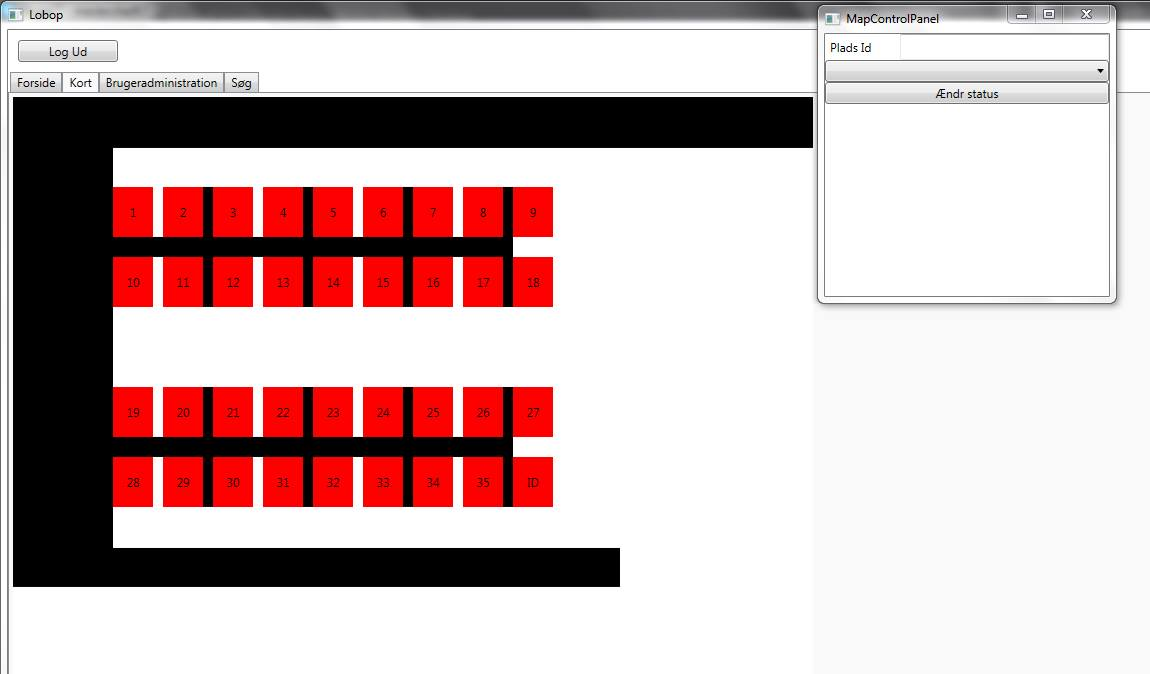
\includegraphics[scale=0.5, angle=270]{lobopkort.jpg}
  \caption{Kort funktion fra LOBOP}
  \label{fig:lobopkort}
\end{figure}


Programmets hovedfunktioner såsom brugeradministration, visning af kort\cref{fig:lobopkort} og søgefunktionaliteten fungererer efter hensigten, se \cref{sec:moduler}. Udover disse funktioner, mangler eller kan følgende funktioner forbedres. Chiplæseren ved login, er simuleret som et tekstfelt i brugergrænsefladen. Denne funktionalitet kan med fordel erstattes af en rigtig hardware chiplæser. En anden funktion der kan tilføjes til programmet er muligheden for at ændre brugertilladelserne ved programkørselstid. Derudover bliver hver bådplads sensor simuleret ved software. Det vil sige at sensoren kan styres fra programmet. En forbedring af denne funktionalitet, ville være at en rigtig hardware sensor bruges i stedet for den simulerede sensor.

%Programmet består af en brugergrænseflade, som inderholder fire faner med hver deres ansvarsområde. Den første fane er forsiden, som ikke indeholder funktionalitet, udover en beskrivelse af hvordan programmet bruges.


%Næste fane er kort funktionen, som viser et kort over en prædefineret havn. På fanen her er det muligt at se status på alle havnens pladser. Fra kortet er det også muligt at sende brugeren videre til brugeradministrationsfanen, ved at venstre klikke på en plads. Højere klikkes der på en plads vil pladsens oplysninger blive vist i et nyt vindue hvor det her er muligt at ændre pladsens egenskaber.

%Brugeradministrations fanen har til formål at vise informationer om en bruger, samt gøre det muligt at ændre i en brugers egenskaber. På siden er vist brugerens egenskaber og en liste af personens både. I listen er det muligt at vælge en båd og derved få vist bådens egenskaber.
